Neuschnee verändert sich in einer Schneemetamorphose. Bei der Metamorphose sublimiert Wasserdampf und lagert sich an einer anderen Stelle wieder an. Die Geschwindigkeit der Umwandlung ist je nach Umgebungsbedingunen sehr unteschiedlich. Die Temperatur in Schnee ist relativ konstant 0 grad.

Mit der Methamrophose ändern sich die Eigenschafetn des schnees. Grundprinzipien bei der Methamorphose sind zum Beispiel der Trieb die Oberfläche zu verkleinern, dass heisst das Material feine Eisästchen gehen zu konkaven Mulden.

Bei der Schmelzmetamorphose entsteht im Porenraum des Schnees Schmelzwasser. Die Umwandlung zu runden Strukturen geht besonders schnell vorran.

\begin{figure}[H]
    \centering
    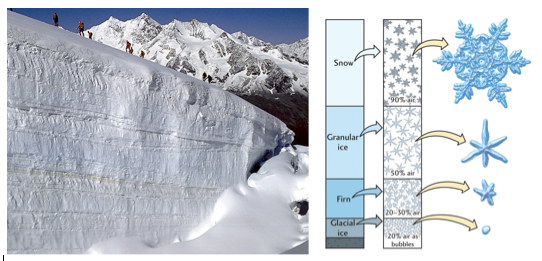
\includegraphics[width=0.8\textwidth]{Bilder/gletscher_eis_schnee.png}
    \caption{Abbildung von Schnee Methamorphose}
    \label{fig:Metha}
\end{figure}